\documentclass[compress]{beamer}

\usepackage{tikz} % Pretty pictures, google tikzmanual.pdf
\usetikzlibrary{arrows,decorations.pathmorphing,decorations.markings,backgrounds}
\usepackage{pgfplots}

\tikzstyle{vecArrow} = [thick, decoration={markings,mark=at position
   1 with {\arrow[semithick]{open triangle 60}}},
   double distance=1.4pt, shorten >= 5.5pt,
   preaction = {decorate},
   postaction = {draw,line width=1.4pt, white,shorten >= 4.5pt}]
\tikzstyle{innerWhite} = [semithick, white,line width=1.4pt, shorten >= 4.5pt]

\usepackage{amsmath}
\usepackage{eepic}
\usepackage{epic}
\usepackage{epsfig}
\usepackage{moreverb}
\usepackage{stfloats}
\usepackage{algorithm}
\usepackage{amsthm}
\usepackage{algpseudocode}
\usepackage{amsthm}
\usepackage{multicol}

\usetheme{Warsaw}
\usepackage{multicol}

\colorlet{mycolor}{orange!80!black}% change this color to suit your needs

\AtBeginSection[]{
  \setbeamercolor{section in toc shaded}{use=structure,fg=structure.fg}
  \setbeamercolor{section in toc}{fg=mycolor}
  \setbeamercolor{subsection in toc shaded}{fg=black}
  \setbeamercolor{subsection in toc}{fg=mycolor}
  \frame<beamer>{
    \begin{multicols}{2}
      \frametitle{Outline}
      \setcounter{tocdepth}{2}  
      \tableofcontents[currentsection,subsections]
    \end{multicols} 
  }
}

\setbeamercolor{author in head/foot}{fg=white}
\setbeamercolor{title in head/foot}{fg=mycolor}
\setbeamercolor{section in head/foot}{fg=mycolor}
\setbeamertemplate{section in head/foot shaded}{\color{white!70!black}\insertsectionhead}
\setbeamercolor{subsection in head/foot}{fg=mycolor}
\setbeamertemplate{subsection in head/foot shaded}{\color{white!70!black}\insertsubsectionhead}
\setbeamercolor{frametitle}{fg=white}
\setbeamercolor{framesubtitle}{fg=white}

\title{One Dimensional Algorithmic Questions}
\author{James Zuber}
\institute{Stony Brook University}
\date{\today}


\begin{document}

\begin{frame}
  \maketitle
\end{frame}

\section[Airplane Seating]{Airplane Seating}
\begin{frame}\frametitle{1-Dimensional Airplanes}

\begin{figure}[H]
\label{fig:lineplane}
\centering
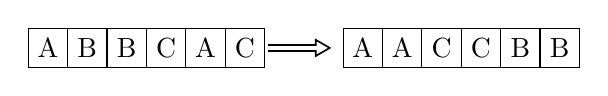
\begin{tikzpicture}[scale=1]
\draw (0,0.0) +(-.25,-.25) rectangle ++(.25,.25);
\draw (0,0.0) node{A};
\draw (0.5,0) +(-.25,-.25) rectangle ++(.25,.25);
\draw (0.5,0) node{B};
\draw (1.0,0) +(-.25,-.25) rectangle ++(.25,.25);
\draw (1.0,0) node{B};
\draw (1.5,0) +(-.25,-.25) rectangle ++(.25,.25);
\draw (1.5,0) node{C};
\draw (2.0,0) +(-.25,-.25) rectangle ++(.25,.25);
\draw (2.0,0) node{A};
\draw (2.5,0) +(-.25,-.25) rectangle ++(.25,.25);
\draw (2.5,0) node{C};

\visible<2-3>
{
\draw[vecArrow] (2.8,0) to (3.6,0);

\draw (4,0.0) +(-.25,-.25) rectangle ++(.25,.25);
\draw (4,0.0) node{A};
\draw (4.5,0) +(-.25,-.25) rectangle ++(.25,.25);
\draw (4.5,0) node{A};
\draw (5.0,0) +(-.25,-.25) rectangle ++(.25,.25);
\draw (5.0,0) node{C};
\draw (5.5,0) +(-.25,-.25) rectangle ++(.25,.25);
\draw (5.5,0) node{C};
\draw (6.0,0) +(-.25,-.25) rectangle ++(.25,.25);
\draw (6.0,0) node{B};
\draw (6.5,0) +(-.25,-.25) rectangle ++(.25,.25);
\draw (6.5,0) node{B};
}
\end{tikzpicture}
\end{figure}

\visible<3>
{
Important features:

\begin{itemize}
\item Airplane only has 1 long row of seats.
\item All family members identical.
\item No preferred sort order (ABC as good as CAB).
\item Can only swap 2 passengers at a time.
\end{itemize}
}
\end{frame}

\begin{frame}\frametitle{Hardness}
Given a set of $n = 3m$ integers $x_i$, is there a grouping of the $x_i$ into $m$ disjoint triplets so that the sum of each triplet is the same number $k$?  

Gadgets:
\visible<2->
{
Large blocking families $B_j$ between each $k$-width seating area.
}

\visible<3->
{
A family of $f_i$ with $x_i$ members for each $x_i$.
}

\visible<4->
{
One seatwarmer family $S$ at end of plane.
}


Starting position:

\begin{figure}[H]
\centering
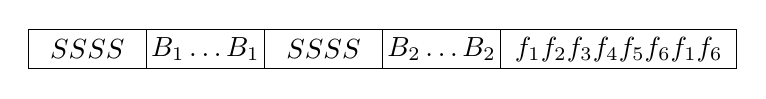
\begin{tikzpicture}[scale=1]
\draw (0,0.0) +(-.75,-.25) rectangle ++(.75,.25);
\visible<4->
{
\draw (0,0.0) node{$SSSS$};
}
\draw (1.5,0) +(-.75,-.25) rectangle ++(.75,.25);
\visible<2->
{
\draw (1.5,0) node{$B_1 \hdots B_1$};
}
\draw (3,0) +(-.75,-.25) rectangle ++(.75,.25);
\visible<4->
{
\draw (3,0) node{$SSSS$};
}
\draw (4.5,0) +(-.75,-.25) rectangle ++(.75,.25);
\visible<2->
{
\draw (4.5,0) node{$B_2 \hdots B_2$};
}
\draw (6.75,0) +(-1.5,-.25) rectangle ++(1.5,.25);
\visible<3->
{
\draw (6.75,0) node{$f_1 f_2 f_3 f_4 f_5 f_6 f_1 f_6$};
}
\end{tikzpicture}
\end{figure}

Final position (only achieveable in $mk$ swaps if there is a 3-partition)

\begin{figure}[H]
\centering
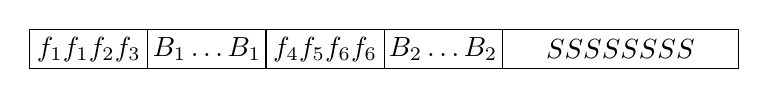
\begin{tikzpicture}[scale=1]
\draw (0,0.0) +(-.75,-.25) rectangle ++(.75,.25);
\visible<3->
{
\draw (0,0.0) node{$f_1 f_1 f_2 f_3$};
}
\draw (1.5,0) +(-.75,-.25) rectangle ++(.75,.25);
\visible<2->
{
\draw (1.5,0) node{$B_1 \hdots B_1$};
}
\draw (3,0) +(-.75,-.25) rectangle ++(.75,.25);
\visible<3->
{
\draw (3,0) node{$f_4 f_5 f_6 f_6$};
}
\draw (4.5,0) +(-.75,-.25) rectangle ++(.75,.25);
\visible<2->
{
\draw (4.5,0) node{$B_2 \hdots B_2$};
}
\draw (6.75,0) +(-1.5,-.25) rectangle ++(1.5,.25);
\visible<4->
{
\draw (6.75,0)node{$SSSSSSSS$};
}
\end{tikzpicture}
\end{figure}

\end{frame}

\begin{frame}{Greedy Algorithm}

We showed that, for a plane filled with couples, the simplest sweep algorithm is optimal due to the following observation:

\begin{figure}[H]
\centering
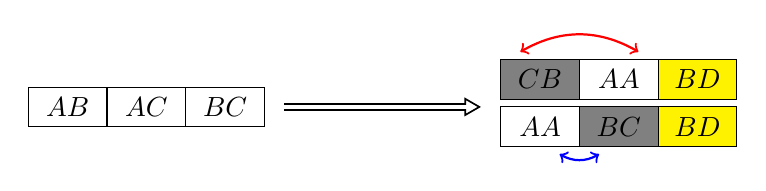
\begin{tikzpicture}[scale=1]
\draw (-6.0,0.25) +(-.5,-.25) rectangle ++(.5,.25);
\draw (-6.0,0.25) node{$A B$};x
\draw (-5.0,0.25) +(-.5,-.25) rectangle ++(.5,.25);
\draw (-5.0,0.25) node{$A C$};
\draw (-4.0,0.25) +(-.5,-.25) rectangle ++(.5,.25);
\draw (-4.0,0.25) node{$B C$};

\draw[vecArrow] (-3.25,0.25) to (-0.75,0.25);

\visible<2>
{
      \draw [thick,red,bend left,<->] (-0.25,0.95) to (1.25,0.95);
}

\visible<4->
    {
      \fill[gray] (0.0,.60) +(-.5,-.25) rectangle ++(.5,.25);
      \fill[gray] (1.0,0) +(-.5,-.25) rectangle ++(.5,.25);

      \fill[yellow] (2.0,.60) +(-.5,-.25) rectangle ++(.5,.25);
      \fill[yellow] (2.0,0) +(-.5,-.25) rectangle ++(.5,.25);

    }

\visible<2->
    {
       \draw (0.0,.60) +(-.5,-.25) rectangle ++(.5,.25);
       \draw (0.0,.60) node{$C B$};
       \draw (1.0,.60) +(-.5,-.25) rectangle ++(.5,.25);
       \draw (1.0,.60) node{$A A$};
       \draw (2.0,.60) +(-.5,-.25) rectangle ++(.5,.25);
       \draw (2.0,.60) node{$B D$};
    }
\visible<3>
{
      \draw [thick,blue,bend right,<->]  (0.25,-0.35) to (0.75,-0.35);
}
\visible<3->
    {
      \draw (0,0.0) +(-.5,-.25) rectangle ++(.5,.25);
      \draw (0,0.0) node{$A A$};
      \draw (1.0,0) +(-.5,-.25) rectangle ++(.5,.25);
      \draw (1.0,0) node{$B C$};
      \draw (2.0,0) +(-.5,-.25) rectangle ++(.5,.25);
      \draw (2.0,0) node{$B D$};
    }
\end{tikzpicture}
\end{figure}

\only<2>
{
The {\color{red}{red} exchange.}
}

\only<3>
{
And the {\color{blue}{blue} exchange.}
}

\only<4>
{
Leave the remaining passengers' seating locations equivalent.
}


\end{frame}

\begin{frame}\frametitle{Mixed Couples and Singles: Alignment}



\begin{figure}[H]
\centering
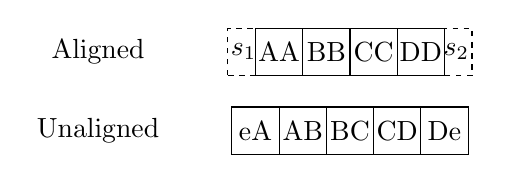
\begin{tikzpicture}[scale=1]
\draw (-2,1) node{Aligned};
\draw[dash pattern= on 2pt off 2pt] (-0.15,1) +(-.2,-.3) rectangle ++(.15,.3);
\draw (-0.15,1) node{$s_1$};
\draw (0.3,1) +(-.3,-.3) rectangle ++(.3,.3);
\draw (0.3,1) node{AA};
\draw (0.9,1) +(-.3,-.3) rectangle ++(.3,.3);
\draw (0.9,1) node{BB};
\draw (1.5,1) +(-.3,-.3) rectangle ++(.3,.3);
\draw (1.5,1) node{CC};
\draw (2.1,1) +(-.3,-.3) rectangle ++(.3,.3);
\draw (2.1,1) node{DD};
\draw[dash pattern= on 2pt off 2pt] (2.55,1) +(-.15,-.3) rectangle ++(.2,.3);
\draw (2.55,1) node{$s_2$};

\draw (-2,0) node{Unaligned};
\draw (0.0,0) +(-.3,-.3) rectangle ++(.3,.3);
\draw (0.0,0) node{eA};
\draw (0.6,0) +(-.3,-.3) rectangle ++(.3,.3);
\draw (0.6,0) node{AB};
\draw (1.2,0) +(-.3,-.3) rectangle ++(.3,.3);
\draw (1.2,0) node{BC};
\draw (1.8,0) +(-.3,-.3) rectangle ++(.3,.3);
\draw (1.8,0) node{CD};
\draw (2.4,0) +(-.3,-.3) rectangle ++(.3,.3);
\draw (2.4,0) node{De};
\end{tikzpicture}
\end{figure}
\end{frame}

\section[DNA]{Genetic Intervals}
\begin{frame}\frametitle{DNA Copy Analysis}
\end{frame}

\section[Waiter]{Waiter Problem}
\begin{frame}\frametitle{Don't Drop that Tray}

\end{frame}

\end{document}

